\subsection{Principles}
\begin{defnbox}\nospacing
  \begin{defn}[Encapsulation]\label{defn:encapsulation}\leavevmode
    \begin{itemizenosep}
      \item Methods and data are combined in classes
      \item Not unique to OOP
    \end{itemizenosep}
  \end{defn}
\end{defnbox}
\subsection{Class Basics}
\subsubsection{Static}
\label{subsubsec:Static}
\begin{defnbox}\nospacing
  \begin{defn}[Static Fields]\label{defn:staticFields}
    Per class fields, accessible via class (or instance)
    \begin{itemizenosep}
        \item Bound to class (available even if no instance has been created)
        \item Only one copy of the attribute (identical for all instances)
        \item Initialization per default with zero (0 / 0.0 / false / null) 
    \end{itemizenosep}
    \begin{mintlinebox}{java}
      static Type ref;
    \end{mintlinebox}
  \end{defn}
\end{defnbox}
\begin{stylebox}[Constants]\nospacing
  Declare constants as \javainline/static final/ fields.
\end{stylebox}
\begin{defnbox}\nospacing
  \begin{defn}[Static Methods]\label{defn:staticFields}
    Per Class methods, accessible via class (or instance):
    \begin{mintlinebox}{java}
      static ResultType Name(args){ Body }
    \end{mintlinebox}
    \begin{itemizenosep}
        \item No \javainline/this/
        \item No access to instance attributes \& methods
    \end{itemizenosep}
  \end{defn}
\end{defnbox}
\begin{stylebox}\nospacing
  Do not use instances to access static fields or methods.
\end{stylebox}
\subsubsection{Class Initialization}
\begin{sectionbox}[Upon loading o the class]\nospacing
  
\end{sectionbox}
\subsection{Inheritance}
\begin{defnbox}\nospacing
  \begin{defn}[\tc{black}{\normalfont{(Implementation Aspect)}}
    \\Code Inheritance\blacksl Extension\blacksl Subclassing]\leavevmode
    \begin{itemizenosep}
        \item Subclasses add new fields \& methods
        \item Subclasses have more (specialized) attributes \& operations
        \item Implementation aspect
    \end{itemizenosep}
    \imp{Class}: defines a type \imp{and} implementation
  \end{defn}
\end{defnbox}
\begin{defnbox}\nospacing
  \begin{defn}[\tc{black}{\normalfont{(Design Aspect)}}
    \\Interface Inheritance\blacksl Specialization\blacksl Subtyping]\leavevmode
    \begin{itemizenosep}
        \item Types define a set of objects
        \item Subtypes are specializations of this Type
        \item Inheritance of behavioral aspects
    \end{itemizenosep}
    \imp{Interface}: defines type
  \end{defn}
\end{defnbox}
\begin{defnbox}\nospacing
  \begin{defn}[\javainline/extends/]\label{defn:extends}\leavevmode\\
    Define new class by extending existing classes.\\
    In Java only one base class can be specified to inherit from.
    Extension inherits all fields and methods from the base class.
  \end{defn}
\end{defnbox}
\subsubsection{Polymorphism}
\begin{defnbox}\nospacing
  \begin{defn}[Type Checking]
    The process of verifying and enforcing the constraints of types
  \end{defn}
\end{defnbox}
\begin{defnbox}\nospacing
  \begin{defn}[Statically Typed Languages]
    Is a language where the type of a variable is known at compile time.\\
    For some languages this means that we as programmer must specify of what type each variable is.\\
    \Advantage\ can do type-checking during compile time by the compiler, and therefore a lot of trivial bugs are caught at a very early stage.\\
    \imp{Examples}: C, C++, Java
  \end{defn}
\end{defnbox}
\begin{defnbox}\nospacing
  \begin{defn}[Dynamically Typed Languages]
     If the type is associated with/depends on run-time \imp{values}, and not named variables/fields/etc\\
     \Advantage\ we do not have to specify types every time.\\
     \Drawback\ do type checking at run-time
  \end{defn}
\end{defnbox}
\label{subsubsec:Polymorphism}
\begin{defnbox}\nospacing
  \begin{defn}[Polymorphism]\label{defn:polymorphism}
    Polymorphism allows operations to be performed on objects without needing to know which class the object belongs to,
    provided that we can guarantee that the class implements the specified type.
  \end{defn}
\end{defnbox}
\begin{defnbox}\nospacing
  \begin{defn}[Polymorphic Assignment]
    Instances of an extended class can be assigned to references of type base
    class:
    \begin{mintlinebox}{java}
      BaseClass ref = new extendedClass();
    \end{mintlinebox}
  \end{defn}
\end{defnbox}
\begin{defnbox}\nospacing
  \begin{defn}[Dynamic Type]\label{defn:dynamicType}
    Is the type of the object assigned to a reference variable.\\
    Dynamic types of reference variables may change with every assignment.\\
    $\text{Dynamic Type}\subseteq\text{Static Type}$ as the dynamic type most
    full fill at least the guarantees of the static type.
  \end{defn}
\end{defnbox}
\begin{defnbox}\nospacing
  \begin{defn}[Static Binding]
    Is type resolution based on the static type of a variable reference.
  \end{defn}
\end{defnbox}
\begin{defnbox}\nospacing
  \begin{defn}[Static Binding and Overloading]
    If we overload a method in Java, the compiler will produce a version for
    each overloaded function \rd{signature}.\\
    The resolution of the method signature (not to the actual implementation) of the
    method is done during compile time and does hence depend on the \rd{static type}
    passed to the method $\Rightarrow$ static binding
    \begin{mintlinebox}{java}
      StaticTypeOfa a = new DynamicTypeOfa();
      a.methodToResolveTo(StaticTypeOfb b);
    \end{mintlinebox}
    \javainline/staticTypeOfb/ decides which overloaded method to call.
  \end{defn}
\end{defnbox}
\begin{defnbox}\nospacing
  \begin{defn}[\\Dynamic Type Binding and Overloading]
    The runtime chooses a function implementation
    \begin{numberlistnosep}
        \item Based on the function \rd{signature} chosen at compile time
      (dynamic binding)
        \item Depending on the dynamic type of the object referenced by
      \javainline/a/ in order to chose an actual implementation of
      \begin{mintlinebox}{java}
          DynamicTypeOfa.methodToResolveTo(StaticTypeOfb b)
      \end{mintlinebox}
    \end{numberlistnosep}
  \end{defn}
\end{defnbox}
\begin{notebox}[Note]\nospacing
  For non-overloaded methods only the dynamic type of the reference variable
  decides which method to call.
\end{notebox}
\begin{codeboxNl}[Dynamic Type Inference]{java}
  if( ref instanceof Type)
\end{codeboxNl}
\begin{codeboxcomment}[Type Casts]{0.3}{java}{
    A runtime error is thrown if the dynamic type of \javainline/ref/ is not a
    Type or extension thereof.
  }
  (Type) ref;
\end{codeboxcomment}
\subsection{Abstract Classes}
\begin{defnbox}\nospacing
  \begin{defn}[Abstract Methods]
    Are methods that only define a signature/are only a declaration:
    \begin{mintlinebox}{java}
      visibility abstract retrunType methodName();
    \end{mintlinebox}
    \begin{itemizenosep}
        \item Define methods to be implemented in subclasses
        \item Can only be declared in \javainline/abstract/ classes
        \item Cannot be \javainline/private/ as private methods cannot be overridden
        \item Cannot be \javainline/static/ as static methods cannot be overridden
    \end{itemizenosep}
  \end{defn}
\end{defnbox}
\begin{defnbox}\nospacing
  \begin{defn}[Abstract Classes]
    Are classes that how stand in an ``\rd{is-a}'' relationship with their subclasses:
    \begin{itemizenosep}
      \item Cannot be instantiated
      \item Usually have one or more abstract methods
      \item May have attributes, constructors, non-abstract methods 
    \end{itemizenosep}
    \begin{mintlinebox}{java}
      visibility abstract class Name{ Body }
    \end{mintlinebox}
  \end{defn}
\end{defnbox}
\begin{notebox}[Note]\nospacing
  An abstract class must not necessarily have an abstract method.\\
  Useful to declare classes abstract that cannot/may not be initiated but (but extended)
\end{notebox}
\begin{notebox}[Note: \normalfont{Derived Classes}]\nospacing
  \begin{itemizenosep}
      \item Have to override (implement) all \javainline/abstract/ methods
      \item Or have to be declared abstract as well, if not all abstract methods
    are overridden.
  \end{itemizenosep}
\end{notebox}
\begin{notebox}[Note]\nospacing
  Arrays of an abstract base type may be instantiated sine No instances are
  created (only reference variables)
  \begin{mintlinebox}{java}
    ContainerType[] name = new ContainerType[Number]
  \end{mintlinebox}
\end{notebox}
\begin{stylebox}[Usage]\nospacing
  \begin{itemizenosep}
      \item Want to share code among several closely related classes.
      \item You expect that classes that extend your abstract class have many
    common methods or fields or require access modifiers other than public (such
    as protected and private).
      \item You want to declare non-static or non-final fields. This enables you to define methods that can access and modify the state of the object to which they belong.
  \end{itemizenosep}
\end{stylebox}
\subsection{Interfaces}
\begin{defnbox}\nospacing
  \begin{defn}[Interfaces=pure abstract class]\label{defn:interfaces}
    Have to be implemented by the class that uses the interface and represent a
    ``\rd{can-do}'' relationship:
    \begin{itemizenosep}
      \item Have only \javainline/public/ and \javainline/abstract/ methods
      \item Attributes are by default \javainline/public,static/ and
    \javainline/final/
      \item No constructors $\Rightarrow$ instantiated ($\neq$ declared)
    \end{itemizenosep}
    \imp{Definition}:
    \begin{mintlinebox}{java}
      public intreface ClassName{ Body; }
    \end{mintlinebox}
    \imp{Implementation}:
    \begin{mintlinebox}{java}
      class ClassName implements IntefaceName{ Body; }
    \end{mintlinebox}
    \begin{itemizenosep}
        \item All methods defined in the declared interface have to be
      implemented unless its another interface adding more functionality
        \item A class may implement multiple interfaces
    \end{itemizenosep}
  \end{defn}
\end{defnbox}
\begin{notebox}[Note: Java 8 default methods]\nospacing
  Can be implemented inside interfaces and are able access other methods.
  Allows to extend interfaces without breaking existing classes that implement
  the interface.
\end{notebox}
\begin{stylebox}\nospacing
  Use \javainline/@override/ to implement the methods.
\end{stylebox}
\begin{stylebox}[Usage]\nospacing
  \begin{itemizenosep}
    \item You expect that unrelated classes would implement a piece of
  functionality. 
    \item Want to specify the behavior of a particular data type, but not concerned about who implements its behavior.
  \end{itemizenosep}
\end{stylebox}
\begin{notebox}[Interfaces as function arguments]\nospacing
  Methods with Interfaces as type can be called with any class implementation
  that interface.
\end{notebox}
\begin{notebox}[Interface Reference]\nospacing
  Interfaces can be used as reference variable for all subclasses \imp{but} be
  care-full if the reference object implements another interface we will not be
  able to call its functions unless we use an implicit cast.\\
  Check if referenced object implements an interface: \javainline/ref instanceof aInterface/
\end{notebox}
\begin{codeboxNl}[Interaface Variable]{java}
  TypeImplementingAandB ref = new TypeImplementingAandB()
  InterfaceTypeA refA = ref;
  InterfaceTypeB refB = ref;
  refA instanceof InterfaceTypeB // True as ref implements B
  refA.methodOfTypeImplementingAandB() // works
  refA.methodOfB() // does not work
  ((InterfaceTypeB)refA).methodOfB() // works
\end{codeboxNl}
\begin{sectionbox}[Intrefaces and Abstract Classes]\nospacing
  \begin{itemize}
      \item \javainline/Interface/: provides a type
      \item \javainline/abstract Class/ semi finished component that contains
    default implementations
    \begin{itemizenosep}
        \item which can be used in subclasses
        \item which can be overriden in subclasses
    \end{itemizenosep}
  \end{itemize}
  \begin{figure}[H]
    \centering
    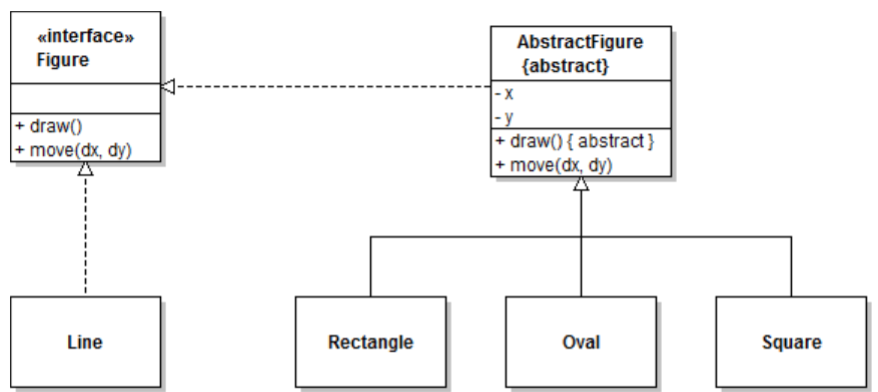
\includegraphics[width=1.0\textwidth]{java/figures/oop/abstractInterface.png}
  \end{figure}
\end{sectionbox}
\begin{notebox}[Abstract Classes vs. Interfaces]\nospacing
  \begin{itemizenosep}
      \item Abstract Classes
    \begin{itemizenosep}
        \item A class may extend only one abstract class
        \item Abstract classes may contain attributes \& concrete implementations
    \end{itemizenosep}
      \item Interfaces
    \begin{itemizenosep}
        \item A class may implement sever interfaces
        \item Abstract classes may contain no implementations 
    \end{itemizenosep}
  \end{itemizenosep}
\end{notebox}
\begin{defnbox}\nospacing
  \begin{defn}[Marker Interface]\label{defn:markerInerface}
    Is an empty interface, that can be used to add a certain
    attribute/characteristic to a class that can be checked with
    \javainline/instanceof/ e.g.\ RandomAcess 
  \end{defn}
\end{defnbox}
\begin{defnbox}\nospacing
  \begin{defn}[Functional Interface \javainline/@FunctionalInterface/]\label{defn:functionalInterface}
    Is an interface with a single abstract method:
    \begin{mintlinebox}{java}
      @FunctionalInterface
      public interface InterfaceName{
        visibility returnType methodName(args);
      }
    \end{mintlinebox}
  \end{defn}
\end{defnbox}
\begin{notebox}[Notes]\nospacing
  \begin{itemizenosep}
      \item The annotation \javainline/@FunctionalInterface/ allows compilers to generate an
  error if the interface does not satisfy the conditions of a functional
  interface.
    \item Default methods are not abstract and do not count.
  \end{itemizenosep}
\end{notebox}
\begin{sectionbox}[Lambda Expressions and Functional Interfaces]\nospacing
  
\end{sectionbox}
%%% Local Variables:
%%% mode: latex
%%% TeX-master: "../../formulary"
%%% End:
